% id: 114-51
% book: 100발100중 3-2 중간 · 01 3-2 중간(삼각비·삼각비의 활용·원과 직선·원주각·부록)
% section: 족집게 마무리 객관식 80선
% figure: crop:fig-114-51.png
% answer: ①
% answer_source: 답지(빠른정답)
% variant_level: 0 (원본 전사)
% 이 파일은 build.mjs 가 items.json 에서 만든다. 고칠 때는 items.json 을 고친다.
\smash{\raisebox{1.5mm}{\dmkichul{100발100중 3-2 중간 114쪽 51번}}}
\noindent\begin{minipage}[t]{0.58\linewidth}\vspace{0pt}\raggedright 그림에서 $\seg{PA}$, $\seg{PB}$는 원~$\pt{O}$의 접선이고 두 점~$\pt{A}$, $\pt{B}$는 접점이다. $\seg{AP}=14\mkern3mu \mathrm{cm}$일 때, 다음 중 옳지 \underline{않은} 것은?\end{minipage}\hfill\begin{minipage}[t]{0.4\linewidth}\vspace{0pt}\centering 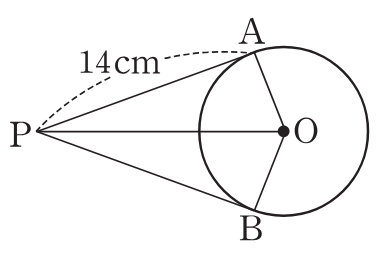
\includegraphics[width=90.1pt]{figures/fig-114-51.png}\end{minipage}\par
\begin{choicesii}{$\seg{OA}=7\mkern3mu \mathrm{cm}$}{$\seg{PB}=14\mkern3mu \mathrm{cm}$}{$\angle\pt{POA}=\angle\pt{POB}$}{$\triangle\pt{PAO}\equiv\triangle\pt{PBO}$}{$\angle\pt{APO}+\angle\pt{POA}=90^\circ$}\end{choicesii}
